\documentclass[10pt,a4paper]{article}
\usepackage[margin=1.9cm,headheight=14pt]{geometry}
\usepackage[T1]{fontenc}
\usepackage{lmodern,microtype}
\usepackage[table]{xcolor}
\usepackage{booktabs,tabularx,array,enumitem,tikz,fancyhdr,titlesec}
\usetikzlibrary{arrows.meta,positioning}
\definecolor{navy}{HTML}{12304A}
\definecolor{teal}{HTML}{087E8B}
\definecolor{pale}{HTML}{EDF5F7}
\definecolor{muted}{HTML}{546574}
\usepackage[colorlinks=true,urlcolor=teal,linkcolor=teal]{hyperref}
\hypersetup{pdftitle={RouteMate AI: Architecture and Differentiation},pdfauthor={RouteMate AI Project Team}}
\pagestyle{fancy}\fancyhf{}
\fancyhead[L]{\small\color{muted}ROUTEMATE AI / IMPLEMENTATION OVERVIEW}
\fancyhead[R]{\small\color{muted}05 OCT 2026}
\fancyfoot[L]{\small\color{muted}Hyderabad Metro \quad / \quad Source-backed project brief}
\fancyfoot[R]{\small\thepage}
\renewcommand{\headrulewidth}{0.3pt}
\titleformat{\section}{\Large\bfseries\color{navy}}{\thesection}{0.6em}{}
\titleformat{\subsection}{\normalsize\bfseries\color{teal}}{}{0em}{}
\setlength{\parindent}{0pt}\setlength{\parskip}{0.55em}
\setlist{nosep,leftmargin=1.5em,topsep=0.35em}
\renewcommand{\arraystretch}{1.2}
\newcommand{\code}[1]{\texttt{\small\detokenize{#1}}}
\newcommand{\callout}[1]{\begin{center}\fcolorbox{teal}{pale}{\parbox{0.93\linewidth}{#1}}\end{center}}
\begin{document}

{\small\bfseries\color{teal}PROJECT ARCHITECTURE \quad / \quad TECHNOLOGY \quad / \quad DIFFERENTIATION}
\vspace{0.5em}

{\Huge\bfseries\color{navy}RouteMate AI}\par
{\LARGE\color{navy}How the system works, end to end}\par
{\color{muted}High-level implementation brief based on the current repository.}

\section{The product and its core idea}
RouteMate AI is an AI-assisted journey planner for the Hyderabad Metro. Users can choose stations in a form or describe a trip conversationally, including a deadline or a preference such as fewer line changes. The application returns a map, a timed itinerary, fare estimates and an explanation of the selected route.

The bundled dataset contains \textbf{57 stations across three metro lines}. The distinctive engineering choice is a clear division of responsibilities: \textbf{AI interprets and explains; deterministic graph algorithms calculate the journey}. Route calculations are grounded in the stored network and service model, rather than generated as free-form text.

\subsection{Four layers, one connected application}
\begin{center}
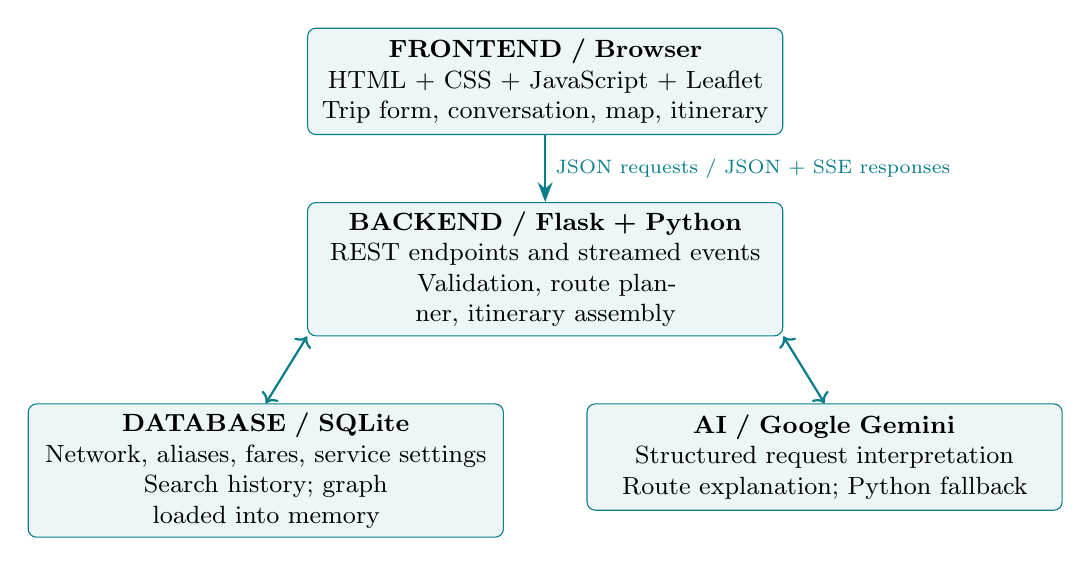
\begin{tikzpicture}[
  box/.style={draw=teal,fill=pale,rounded corners=3pt,text width=5.8cm,minimum height=1.35cm,align=center,font=\small},
  arr/.style={-{Stealth[length=2.5mm]},thick,teal}]
  \node[box] (front) {\textbf{FRONTEND / Browser}\\HTML + CSS + JavaScript + Leaflet\\Trip form, conversation, map, itinerary};
  \node[box,below=0.85cm of front] (back) {\textbf{BACKEND / Flask + Python}\\REST endpoints and streamed events\\Validation, route planner, itinerary assembly};
  \node[box,below left=0.85cm and -2.5cm of back] (db) {\textbf{DATABASE / SQLite}\\Network, aliases, fares, service settings\\Search history; graph loaded into memory};
  \node[box,below right=0.85cm and -2.5cm of back] (ai) {\textbf{AI / Google Gemini}\\Structured request interpretation\\Route explanation; Python fallback};
  \draw[arr] (front.south) -- node[right,font=\scriptsize]{JSON requests / JSON + SSE responses} (back.north);
  \draw[arr,<->] (back.south west) -- (db.north);
  \draw[arr,<->] (back.south east) -- (ai.north);
\end{tikzpicture}
\end{center}

\callout{\textbf{Architecture in one sentence.} The browser calls Flask; Flask uses an in-memory graph loaded from SQLite to compute a route, optionally asks Gemini to interpret or explain it, then returns structured facts for the browser to display.}

\subsection{What this brief establishes}
The following pages describe the implemented request flow, database design, routing and AI boundaries, tools and packages, and the project's defensible strengths. Planned capabilities are identified separately. This is a source and local-test assessment, not a claim of production deployment or live transport accuracy.

\newpage
\section{From a user request to a visible route}
\subsection{Startup: prepare the services once}
Flask's application factory creates the shared services container. Configuration is loaded from environment variables and \code{.env}. SQLite is opened, its schema is created, and the bundled metro JSON is seeded when its SHA-256 digest changes. The database records are loaded into a \code{Network} object; the route planner builds its graph, timetable and station-search index in memory. A Gemini client is configured if AI is enabled.

\subsection{Path A: direct planning through the form}
\begin{enumerate}
\item \textbf{Load the interface.} Flask serves the HTML template and static assets. JavaScript obtains stations, lines, coordinates and available planning modes from \code{GET /api/network}.
\item \textbf{Choose a trip.} Station suggestions come from \code{/api/stations/suggest}; users can also select map stations. The form sends origin, destination, mode, departure/deadline and avoidance settings to \code{GET /api/route}.
\item \textbf{Validate and calculate.} Flask resolves stations and validates the mode and time. The planner searches the graph, evaluates waiting and interchange time, computes fare and constructs the itinerary.
\item \textbf{Return structured facts.} The JSON contains origin/destination, summary metrics, ride/transfer steps, line-coloured geometry, request constraints, notes and search statistics. The backend records the search in SQLite.
\item \textbf{Render the result.} JavaScript updates summary tiles, instructions and Leaflet route polylines. This direct route path does not need a Gemini request.
\end{enumerate}

\subsection{Path B: conversational planning with streaming}
For a request such as \emph{``From Ameerpet to Hitech City before 10, with fewer changes''}, the browser posts \code{text} and previous-trip \code{context} to \code{/api/ask/stream}. It reads Server-Sent Events (SSE) from the response using Fetch; this is a streamed POST response, not a WebSocket connection.

\begin{tabularx}{\linewidth}{@{}l X@{}}
\toprule
\textbf{Stage / event} & \textbf{Backend action and browser effect}\\\midrule
\code{stage} & Signals that request interpretation or explanation is underway.\\
\code{query} / \code{clarify} & Returns validated trip fields, or asks for a missing origin/destination. The browser retains that context for the next message.\\
\code{plan} & Returns the computed itinerary and Pareto options. The map and result can render before the explanation finishes.\\
\code{explanation_delta} & Streams Gemini's explanation text as chunks arrive.\\
\code{explanation} & Supplies the final explanation, including its source: Gemini or template. A fallback can replace incomplete AI text.\\
\code{done} / \code{error} & Completes the request or reports a planning error. Completed/failed planning searches are logged.\\\bottomrule
\end{tabularx}

\subsection{Other connections exposed by the API}
\code{/api/routes/options} returns time/transfer trade-offs; \code{/api/routes/alternatives} provides bounded Yen alternatives; \code{/api/algorithms/compare} returns algorithm statistics and exploration order. \code{/api/health} reports network, graph and AI status. \code{/api/history} exposes recent stored searches. A non-streaming \code{POST /api/ask} is also available.

\newpage
\section{Database and routing engine}
\subsection{SQLite is persistence; the graph is the computation model}
The default database is \code{var/routemate.db}. Python's built-in \code{sqlite3} module uses SQL directly, with foreign keys enabled and WAL journaling for file databases. Network data is loaded at startup, so pathfinding traverses Python objects rather than issuing a database query for every edge. A lock serializes search-log/history access through the shared connection.

\begin{tabularx}{\linewidth}{@{}l X@{}}
\toprule
\textbf{Table} & \textbf{Purpose and relationship}\\\midrule
\code{stations} & Canonical station IDs, names and approximate latitude/longitude.\\
\code{station_aliases} & Alternative names linked to station IDs for lookup and parsing.\\
\code{lines} & Line metadata: colour, corridor and configured total length.\\
\code{line_stations} & Ordered membership connecting stations to lines by sequence.\\
\code{interchanges} & Transfer stations linked to stations, with walking-time assumptions.\\
\code{fare_slabs} & Distance thresholds and fare amounts used by the fare model.\\
\code{meta} & Seed digest, city/timezone, service configuration and fare-source metadata.\\
\code{search_log} & Search channel, text, endpoints, mode, parser, outcome and timing. No user account or saved-trip table is implemented.\\\bottomrule
\end{tabularx}

\subsection{A graph that represents changing trains explicitly}
Each station is expanded into waiting nodes per line and riding nodes per line/direction. Boarding, riding and transferring are distinct edges. Transfers are connected only at configured interchanges, with their walking cost. Temporary source/destination edges are overlaid for each request without copying the entire graph.

\callout{\textbf{Why it matters.} Separating a platform from a train makes waiting time and line changes measurable. A station-only shortest-path graph would need additional logic to represent these constraints faithfully.}

\begin{tabularx}{\linewidth}{@{}p{4.5cm} X@{}}
\toprule
\textbf{Implemented technique} & \textbf{Responsibility}\\\midrule
Time-dependent A* & Default fastest/cheapest search, with a scaled straight-line distance heuristic.\\
Lexicographic Dijkstra & Minimizes transfers, stops or distance first, then arrival time.\\
BFS and 0--1 BFS & Fewest-hop and minimum-transfer algorithm comparisons.\\
Pareto label-setting & Finds non-dominated arrival-time/transfer combinations.\\
Yen's loopless paths & Generates alternative journeys, with request limits and filtering.\\
Binary search & Finds a latest whole-minute departure meeting a deadline within a four-hour search window.\\\bottomrule
\end{tabularx}

\subsection{Time, fare and constraint semantics}
Boarding waits for the next train in a \textbf{modelled} headway schedule. Ride times use calibrated segment distances, running speed and dwell assumptions. Fare is calculated from the shortest track distance between endpoints and the bundled slabs; changing route does not change it in this model. ``Cheapest'' therefore selects the fastest route at the same fare. Avoiding a station prevents boarding/changing there, while trains may still pass through it.

\newpage
\section{AI integration and its boundaries}
\subsection{Understanding: free text becomes a validated trip}
The offline rule parser runs first. It recognizes station names/aliases with the station index, uses cues to identify origin and destination, and extracts preferences and times. When enabled, Gemini also receives the request, station information, current local time and prior-trip context, and returns schema-constrained JSON.

The backend resolves every returned station against the actual network, accepts only supported planning modes and parses time strings. Unknown stations and invalid fields are ignored with notes. Missing Gemini fields can be filled from the rule parse. Prior context fills omitted details in follow-ups; a missing endpoint triggers clarification rather than a fabricated trip.

\subsection{Planning: deterministic computation owns route facts}
The validated trip goes to the same \code{RoutePlanner} used by the form. Gemini does not generate graph edges, pick the path or calculate fares. That separation makes the route calculation repeatable and testable against the network and service assumptions. A valid station choice can still reflect a misunderstood user request; station validation alone does not prove intent was interpreted correctly.

\subsection{Explaining: computed facts become readable guidance}
The explainer builds a compact JSON with line names/directions, endpoints, transfers, departure/arrival, fare, deadline status and alternative options. Gemini is instructed to use only those facts and explain the trip briefly in the chosen language. Input prompts cover English, Telugu, Hindi and mixed-language requests; the explainer also has language mappings for Tamil, Urdu and Kannada.

The prompts constrain narration, but generated prose has \textbf{no independent semantic verification step}. The structured itinerary remains the authoritative calculation. Multilingual quality and landmark-to-station accuracy need representative user testing; the offline parser and template explanation do not provide equivalent multilingual coverage.

\subsection{Fallback and failure handling}
\begin{itemize}
\item A missing API key or disabled AI leaves the rule parser and template explainer available. The direct route form remains usable.
\item An authentication rejection disables the Gemini client for the process. Three transient failures trigger a 60-second cooldown.
\item The configured Gemini request timeout defaults to 45 seconds. Fallback handles failure; it does not guarantee an instant response while a request is pending.
\item If explanation streaming fails, a final template explanation can replace the partial generated text. The already-computed route is retained.
\end{itemize}

\subsection{External services and data movement}
\begin{tabularx}{\linewidth}{@{}l X@{}}
\toprule
\textbf{Service} & \textbf{What crosses the boundary}\\\midrule
Google Gemini & User text, station/context information for parsing; computed route facts for narration. The key stays in backend configuration.\\
OpenStreetMap tiles & Browser requests map tiles for the visible area. The tiles provide a basemap, not routing or live metro data.\\
Leaflet CDN / Google Fonts & Browser downloads the map library/styles and the Inter font. These are additional frontend network dependencies.\\\bottomrule
\end{tabularx}

\callout{\textbf{AI-independent planning is implemented.} Full offline browser operation is not: hosted map tiles, library assets and fonts still require network access unless separately cached or bundled. There is no vector database, RAG pipeline or model training in this implementation.}

\newpage
\section{Tools, packages and custom components}
\subsection{Direct stack and development tooling}
Versions below are resolved in \code{uv.lock}, except Leaflet's template-pinned CDN version. Python's declared minimum is 3.12; the runtime Gemini model is configurable, with \code{gemini-3.1-flash-lite} as the code default, not a guarantee of provider availability.

\begin{tabularx}{\linewidth}{@{}p{4.7cm} X@{}}
\toprule
\textbf{Tool / package} & \textbf{Use in this project}\\\midrule
HTML, CSS, JavaScript & Server-rendered page, layout, application state, Fetch requests and streamed-response handling. No React or Node application layer.\\
Leaflet 1.9.4 + OpenStreetMap & Interactive map, station markers, metro lines and route geometry over an OSM basemap.\\
Google Fonts / Inter & Browser typography loaded from the template.\\
Python $\geq$3.12 & Backend, routing engine, NLP orchestration and command-line entry point.\\
Flask 3.1.3 & Application factory, templates, API blueprint, JSON and SSE responses.\\
google-genai 2.25.0 & Gemini Interactions API calls, JSON responses and text streaming.\\
python-dotenv 1.2.3 & Reads local environment configuration; the loader uses override mode.\\
SQLite / sqlite3 & Embedded relational persistence, seed loading and search history; no separate database server or ORM.\\
pytest 9.1.1 & Algorithm, structure, planner, NLP and Flask test-client checks.\\
uv / uv.lock & Environment/dependency management and reproducible resolved packages.\\
uv\_build & Python packaging backend; declared range $\geq$0.8.23 and $<$0.9.0.\\
Git & Repository version tracking. This review used revision \code{f9c8ee0}.\\\bottomrule
\end{tabularx}

\subsection{Components implemented in the repository}
\textbf{Custom structures:} binary heap, indexed min-heap with decrease-key, directed adjacency-list graph, per-query overlay graph, ranked trie and Damerau--Levenshtein typo matching. \textbf{Custom algorithms:} Dijkstra, A*, BFS, 0--1 BFS, Yen and Pareto search. These are Python modules in the repository, rather than NetworkX or a third-party directions API.

\subsection{Supporting resolved dependencies}
These packages are indirect infrastructure or test dependencies, not separate product features. The complete resolution is recorded in \code{uv.lock}.

{\small
\textbf{Flask/template support:} Werkzeug 3.1.9, Jinja2 3.1.6, MarkupSafe 3.0.3, itsdangerous 2.2.0, blinker 1.9.0, click 8.5.0.

\textbf{HTTP, async and retries:} httpx 0.28.1, httpcore 1.0.9, h11 0.16.0, anyio 4.15.1, sniffio 1.3.1, requests 2.34.2, urllib3 2.8.0, certifi 2026.7.22, charset-normalizer 3.5.1, idna 3.20, websockets 16.1.1, tenacity 9.1.4, distro 1.9.0.

\textbf{Authentication, validation and typing:} google-auth 2.58.1, cryptography 50.0.1, cffi 2.1.1, pycparser 3.0, pyasn1 0.6.4, pyasn1-modules 0.4.2, pydantic 2.13.5, pydantic-core 2.46.5, annotated-types 0.8.0, typing-extensions 4.16.0, typing-inspection 0.4.4.

\textbf{Test/tool support:} iniconfig 2.3.0, pluggy 1.6.0, packaging 26.3, Pygments 2.21.0, colorama 0.4.6. Platform-specific dependencies may not all be installed on every OS.
}

\newpage
\section{How RouteMate differs from existing solutions}
Existing journey planners already offer useful route selection, timing and navigation. RouteMate's case rests on the combination it implements and the ability to inspect its behaviour; route planning or arrival-time selection alone is not a new feature.

\begin{tabularx}{\linewidth}{@{}p{3cm} X X@{}}
\toprule
\textbf{Solution type} & \textbf{Established strength} & \textbf{RouteMate's positioning}\\\midrule
Google Maps & Google's official help documents transit departures and navigation, including schedule information and live departures where provided [1]. & A focused Hyderabad Metro prototype whose graph model, objectives, statistics and algorithm comparisons are directly inspectable in our code/UI.\\
Moovit & Its official trip-planning guide documents route guidance, alternate planning times and live arrival information where available [2]. & Conversational preferences connect to our own deterministic planner, Pareto trade-offs and an AI-independent route path. Broader coverage and live feeds remain advantages of mature transit products.\\
Static metro maps / fare charts & Communicate line layout, interchange locations and fares without an interactive optimization engine. & Adds timed journey computation, station suggestions, route alternatives and readable guidance on top of a stored network.\\
Standalone algorithm visualizers & Typically demonstrate a search method on an abstract graph or grid; this is a category comparison, not an audit of every tool. & Uses a transit graph with line/direction states, waiting, interchange walking, fares and a connected web/API/database workflow.\\
Free-form AI route advice & A general conversational model can describe a journey, but text alone is not evidence that a route was calculated against this project's network. & Route facts come from code and stored data; Gemini assists around that calculation, with station validation and a template fallback.\\\bottomrule
\end{tabularx}

\subsection{Why our implementation stands out}
\begin{enumerate}
\item \textbf{An auditable route calculation.} The project exposes how journeys are found, including algorithm search statistics and comparison traces. This is useful for evaluation, learning and debugging.
\item \textbf{Preferences map to explicit objectives.} ``Fewer changes'' becomes a transfer-first objective; a deadline invokes departure-time search. Pareto options make time-versus-transfer choices visible.
\item \textbf{Conversation is connected to a real engine.} Follow-up context, constrained JSON and station resolution bridge flexible language input to a reproducible calculation.
\item \textbf{Useful when AI is unavailable.} Form planning, rule interpretation and template explanations reduce dependence on a paid/external model for the core journey calculation.
\item \textbf{Compact and understandable implementation.} One Flask application and embedded SQLite keep the prototype simple to run, while custom data structures and algorithms make the engineering contribution clear.
\end{enumerate}

\callout{\textbf{A defensible project pitch.} ``RouteMate AI combines conversational metro planning with an inspectable graph engine. It translates travel preferences into explicit routing objectives, displays the calculated journey and explains the result, while keeping core planning available without AI.''}

This comparison is based on our source and official product documentation, not hands-on competitor testing. It does not establish that these capabilities are unique, or that competitors lack equivalent internal methods. No cross-product speed, cost or accuracy benchmark has been performed.

\newpage
\section{Evidence, present scope and next steps}
\subsection{Local verification}
On 5 October 2026, \code{uv run pytest -q} completed with \textbf{117 passed in 2.05 seconds}. The suite includes algorithm comparisons against brute-force/reference results, heap checks, journey invariants, deadline and avoidance behaviour, fake-Gemini validation/fallback tests and Flask test-client API checks, including SSE. This supports the current implementation; it does not prove live Gemini availability, real transport timing or deployed behaviour.

\subsection{Implemented versus planned}
\begin{tabularx}{\linewidth}{@{}X X@{}}
\toprule
\textbf{Implemented in this checkout} & \textbf{Future work / not established here}\\\midrule
Metro network, graph planning, station lookup, modeled timetable, fare calculation and itinerary/map rendering. & Bus/walking multimodal routing, live train telemetry, disruptions, crowding and least-crowded optimization.\\
Natural-language API, browser-held follow-up context, JSON validation, streamed explanation and fallback. & Voice input, fully localized Telugu/Hindi UI and measured multilingual/landmark accuracy.\\
Algorithm comparison UI/API, exploration-order data and search-history API. & Animated algorithm visualizer, search-history/saved-trip UI, account-based storage.\\
Local CLI, Flask app and test suite. & Verified production deployment, production concurrency/latency measurements and operating costs.\\\bottomrule
\end{tabularx}

\subsection{Assumptions that shape the answer}
\begin{itemize}
\item Station coordinates are approximate. Track segments are scaled to configured line lengths; this is not a surveyed track geometry dataset.
\item Service headways, speed, dwell, access and transfer walking are modeled. Times are estimates from that model, not live arrivals or official train schedules.
\item Fare data is bundled with a source reference to the revised 24 May 2025 chart. Its inclusion does not verify that fares remain current on the review date.
\item ``Optimal'' means optimal for the chosen objective and modeled graph/service assumptions, within applicable search/filter bounds. It is not a guarantee about a real-world journey.
\item Search history stores raw query text in the local database. Conversation context is held in browser state and sent with requests; there is no persistent user-session database model.
\end{itemize}

\subsection{Suggested implementation sequence}
First validate fares, network and service assumptions against current transport information. Then integrate authoritative schedules/live updates and extend the graph for walking/bus legs. In parallel, test multilingual interpretation on representative trips, animate the existing exploration data and add history/saved-trip screens. Production work should measure latency and concurrency before claiming scale or speed advantages.

\subsection{Source map and external references}
{\small
\textbf{Repository evidence:} \code{pyproject.toml}, \code{uv.lock}, \code{src/routemate/web/}, \code{services.py}, \code{db.py}, \code{config.py}, \code{network/}, \code{planner/}, \code{nlp/}, \code{algorithms/}, \code{ds/} and \code{tests/}. Paths after the first web path are relative to \code{src/routemate/}, except \code{tests/}.

\textbf{[1]} Google Maps Help, \href{https://support.google.com/maps/answer/6142130?hl=en-GB}{Get train and bus departures}. Official documentation consulted 5 October 2026.

\textbf{[2]} Moovit Help Center, \href{https://support.moovitapp.com/hc/en-us/articles/212011605-Plan-a-Trip-Get-Directions}{Plan a Trip \& Get Directions}. Official documentation consulted 5 October 2026.

\textbf{Document build:} Authored in LaTeX; compiled using the public \href{https://latex.ytotech.com/builds/sync}{YtoTech LaTeX-on-HTTP API} with \code{pdflatex}. The \href{https://github.com/YtoTech/latex-on-http}{API documentation} describes JSON submission of a main TeX resource. Document tools are separate from the RouteMate runtime stack.
}
\end{document}
